%; whizzy chapter
% -initex iniptex -latex platex -format platex -bibtex jbibtex -fmt fmt
% $B0J>e(B whizzytex $B$r;HMQ$9$k>l9g$N@_Dj(B.

%     Kansai Debian Meeting resources
%     Copyright (C) 2007 Takaya Yamashita
%     Thank you for Tokyo Debian Meeting resources

%     This program is free software; you can redistribute it and/or modify
%     it under the terms of the GNU General Public License as published by
%     the Free Software Foundation; either version 2 of the License, or
%     (at your option) any later version.

%     This program is distributed in the hope that it will be useful,
%     but WITHOUT ANY WARRANTY; without even the implied warranty of
%     MERCHANTABILITY or FITNESS FOR A PARTICULAR PURPOSE.  See the
%     GNU General Public License for more details.

%     You should have received a copy of the GNU General Public License
%     along with this program; if not, write to the Free Software
%     Foundation, Inc., 51 Franklin St, Fifth Floor, Boston, MA  02110-1301 USA

%  preview (shell-command (concat "evince " (replace-regexp-in-string "tex$" "pdf"(buffer-file-name)) "&"))
% $B2hA|%U%!%$%k$r=hM}$9$k$?$a$K$O(B ebb $B$rMxMQ$7$F(B boundingbox $B$r:n@.(B.
%(shell-command "cd image200708; ebb *.png")

%%$B$3$3$+$i%X%C%@3+;O(B.

\documentclass[mingoth,a4paper]{jsarticle}
\usepackage{kansaimonthlyreport}
\usepackage[dvips]{xy}
\usepackage{ascmac}

% $BF|IU$rDj5A$9$k(B, $BKh7nJQ$o$j$^$9(B.
\newcommand{\debmtgyear}{2011}
\newcommand{\debmtgdate}{23}
\newcommand{\debmtgmonth}{01}
\newcommand{\debmtgnumber}{43}

\begin{document}

\begin{titlepage}

% $BKh7nJQ99$9$kItJ,(B, $BK\J8$NKvHx$b=$@5$9$k$3$H$r$o$9$l$:$K(B

 $BBh(B\debmtgnumber{}$B2s(B $B4X@>(B Debian $BJY6/2q;qNA(B

\vspace{2cm}

\begin{center}
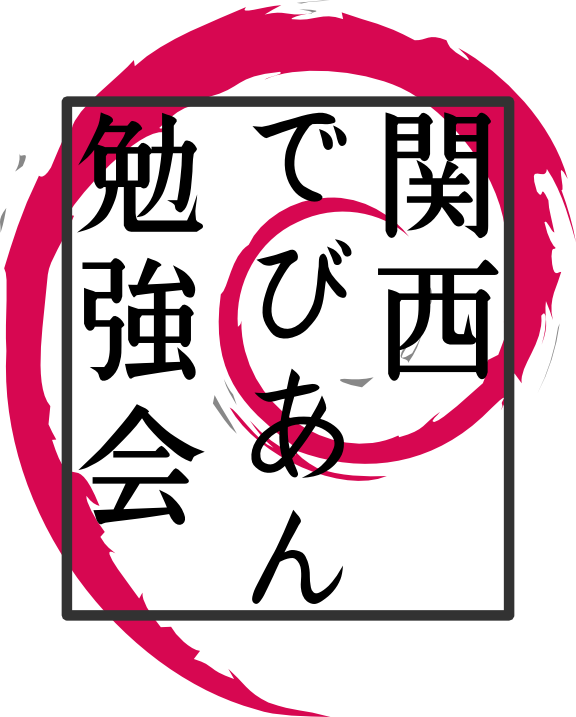
\includegraphics{image200802/kansaidebianlogo.png}
\end{center}

\begin{flushright}
\hfill{}$B4X@>(B Debian $BJY6/2qC4Ev<T(B $B:4!9LZ!&ARI_!&$N$,$?(B \\
\hfill{}\debmtgyear{}$BG/(B\debmtgmonth{}$B7n(B\debmtgdate{}$BF|(B
\end{flushright}

\thispagestyle{empty}
\end{titlepage}

\dancersection{Introduction}{Debian JP}

\subsection*{}%$B%m%4MQ$N%9%Z!<%92T$.(B

$B4X@>(B Debian $BJY6/2q$O(B Debian GNU/Linux $B$N$5$^$6$^$J%H%T%C%/(B ($B?7$7$$%Q%C%1!<(B
$B%8(B, Debian $BFCM-$N5!G=$N;EAH(B, Debian $B3&7($G5/$3$C$?=PMh;v(B, $B$J$I$J$I(B) $B$K(B
$B$D$$$FOC$79g$&2q$G$9(B.

$BL\E*$H$7$F<!$N;0$D$r9M$($F$$$^$9(B.
\begin{itemize}
      \item ML $B$d7G<(HD$G$O$J$/(B, $BD>@\4i$r9g$o$;$k;v$G$N>pJs8r49$NB%?J(B
      \item $BDj4|E*$K=8$^$l$k>l=j(B
      \item $B;qNA$N:n@.(B
\end{itemize}

$B$=$l$G$O(B, $B3Z$7$$0l;~$r$*3Z$7$_2<$5$$(B.

\clearpage

\begin{minipage}[b]{0.2\hsize}
 {\rotatebox{90}{\fontsize{80}{80}
{\gt $B4X@>(B Debian $BJY6/2q(B}}}
\end{minipage}
\begin{minipage}[b]{0.8\hsize}
\hrule
\vspace{2mm}
\hrule
\setcounter{tocdepth}{1}
\tableofcontents
\vspace{2mm}
\hrule
\end{minipage}

\dancersection{$B:G6a$N(B Debian $B4X78$N%$%Y%s%HJs9p(B}{Debian JP}

\subsection{$BBh(B 42 $B2s4X@>(B Debian $BJY6/2q(B}
$BA02s$N4X@>(B Debian $BJY6/2q$O(B 12 $B7n(B 23 $BF|Bg:eJ!Eg6hL1%;%s%?!<$G3+$+$l$^$7$?(B.


\subsection{$BBh(B 71 $B2sEl5~%(%j%"(B Debian $BJY6/2q(B}
2010 $BG/(B 12 $B7n(B 18 $BF|$K3+:E$5$l(B, libsane $B$H(B CACert $B$NOCBj$,$"$C$?$=$&(B. kinnect $B$N%G%b$H$+(B?

\begin{figure}[h!]
  \centering
  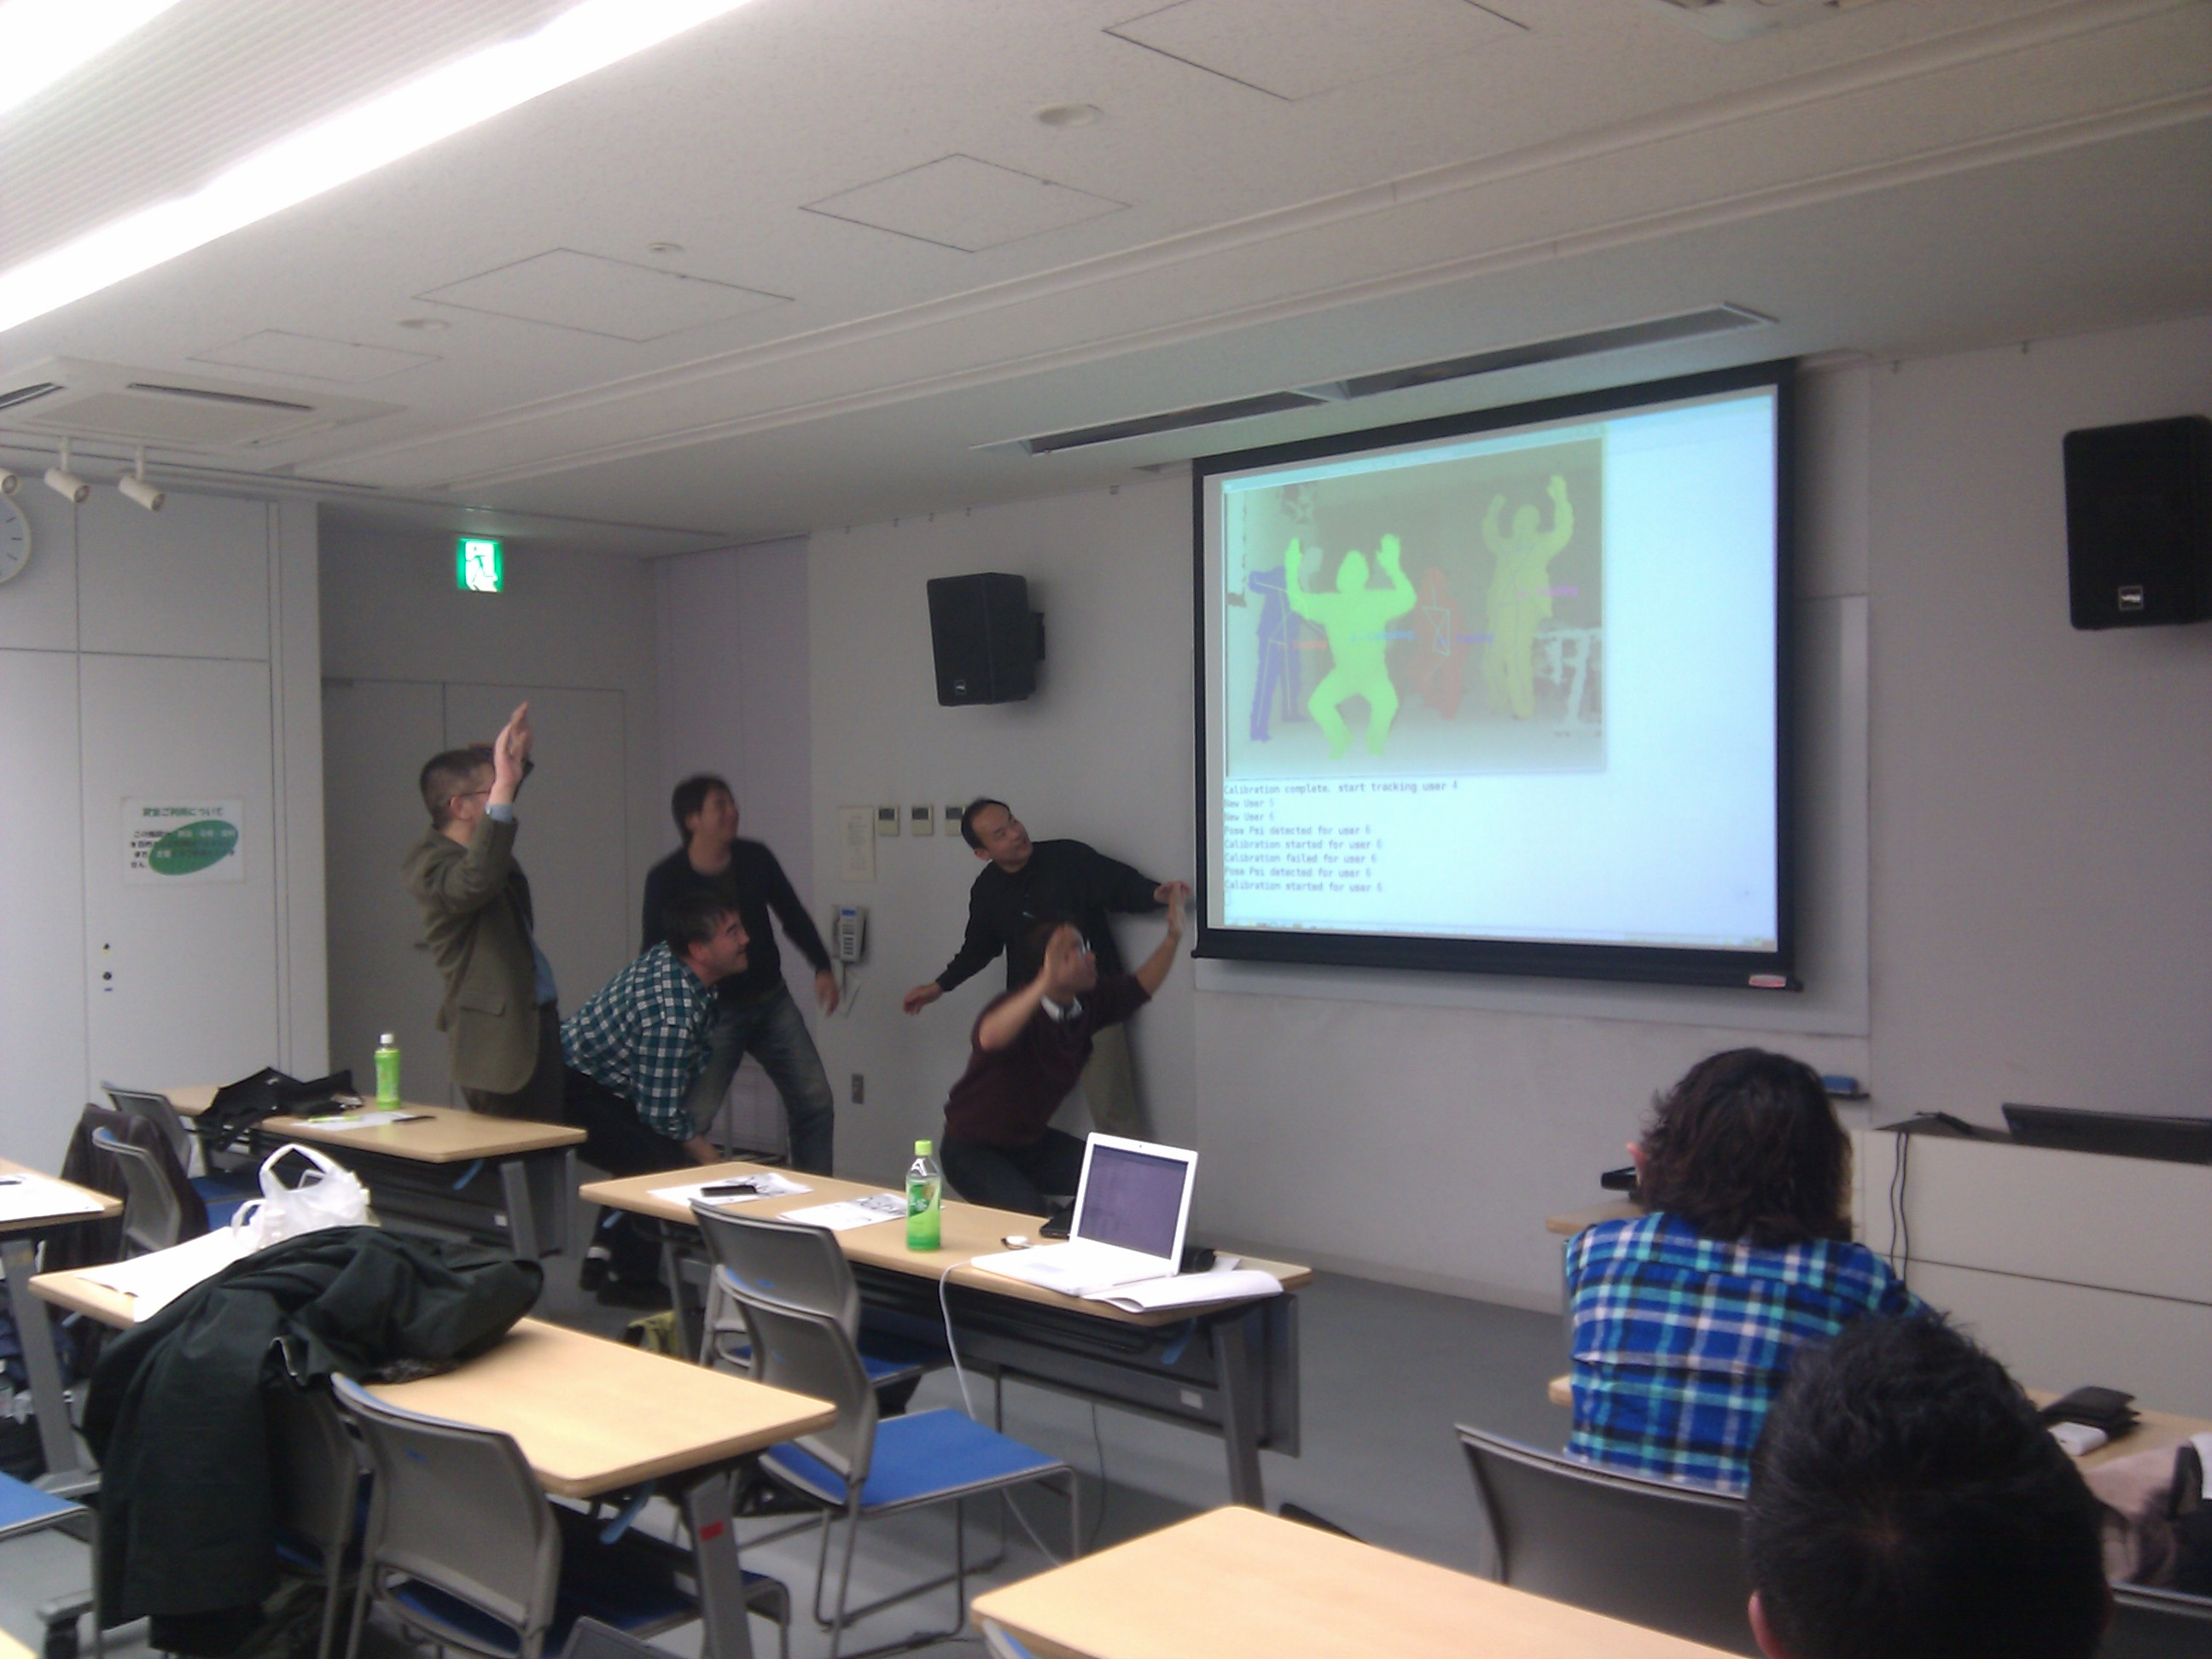
\includegraphics[width=.6\textwidth]{./image201101/kinect.jpg}
  \caption{Kinect $B$GMY$k3'$5$s(B}
  \label{fig:kinect}
\end{figure}


\dancersection{$B;vA02]Bj(B}{Debian JP}

$B:#2s$O0J2<$N2]Bj$r@_Dj$7$^$7$?(B.
%
\begin{quote}
    \begin{screen}
$B0l$D%P%0$r$_$D$1$F$-$F2<$5$$(B. $B$40U8+MWK>$G$b$+$^$$$^$;$s(B.
    \end{screen}
\end{quote}
%
$B;22C<T$N3'$5$s$K$h$k2sEz$O0J2<$NDL$j$G$9(B.
\begin{prework}{ $B:4!9LZMNJ?(B }
  \begin{itemize}
  \item yaskkserv: daemon $B$,F0:n$7$F$$$J$$;~$K(B /etc/init.d/yaskkserv restart $B$9$k$H(B error
  \item howm: howm-vars.el $B$r(B byte-compile $B$9$k$H(B old-style backqoutes
  \item elscreen: emasc22 $B$O(B elscreen $B;H$&$H(B, $B5/F0;~$K%U%!%$%k$,3+$1$^$;$s(B.
    \begin{itemize}
    \item unstable $B$G$O$J$*$C$F$^$9$N$G(B backports $B$7$^$7$g$&(B.
    \end{itemize}
  \item ptex-base,ptex-bin (wishlist): UTF-8 $B$,DL$j$^$;$s(B.
  \end{itemize}
\end{prework}

\begin{prework}{ dpqpqb }

lenny $B$N%7%c%C%H%@%&%sCf$K%O%s%0$9$k>l9g$,M-$k(B.
$B;EJ}L5$7$KEE8;%\%?%s$ND92!$7$GBP=h$7$F$^$9(B.

Debian 5.0.8
Kernel 2.6.26-2-686
GNOME  2.22.3

\end{prework}

\begin{prework}{ $B;32<9/@.(B }

http://www.debian.org/releases/squeeze/armel/apds03.html.ja
D.3.4.1. $B%G%P%$%9%U%!%$%k$N:n@.(B $B$K$O(B,
\begin{commandline}
$B<!$N$h$&$K$7$F(B, $B%G%U%)%k%H$N@EE*%G%P%$%9%U%!%$%k72$r:n@.$7$^$9(B.

# cd /dev
# MAKEDEV generic
\end{commandline}
$B$H$N5-=R$,$"$j$^$9$,(B, $B5-=R$NDL$j$K<B9T$9$k$H(B,
\begin{commandline}
# MAKEDEV generic
.udevdb or .udev presence implies active udev.  Aborting MAKEDEV invocation.
#
\end{commandline}
$B$H$J$j$^$9(B
\end{prework}

\begin{prework}{ $B@n9>(B }

$B%P%0$K$D$$$F$G$9$,(B, $B0JA0$K$bOC$7$?;v$,$"$k$h$&$K%9%/%j%W%H$d%Q%C%1!<%8$,<+J,$N!V0U?^!W$H0[$J$kF0$-$r$7$?$H$-$K(B, $B$=$l$,!V%P%0!W$J$N$+!V@_Dj%_%9!W$J$N$+J,$+$i$J$$$H$-$,$"$j$^$9(B. Xen $B$G8@$($P;~9o$N@_Dj$d(B iptables $B$G(B forward $B$rM-8z$K@_Dj$7$?>l9g$K3F(B DomainU $B$,30It$K@\B3$G$-$J$/$J$k$J$I$G$9(B.
\end{prework}

\begin{prework}{ $B>>_7FsO:(B }

reportbug $B$,%m!<%+%i%$%:$5$l$F$$$J$$(B. gettext $B$N%i%C%T%s%0$5$($7$F$J$5$2(B.
($B$`$7$m0U?^E*(B? $BEvA31Q8l$r;H$($h$J(B, $B$H0E$K$[$N$a$+$7$F$$$k5$$b$9$k(B)
\end{prework}

\begin{prework}{ bpasao }

($BL52sEz(B)

\end{prework}

\begin{prework}{ lurdan }

{\url{http://bugs.debian.org/cgi-bin/bugreport.cgi?bug=607721}}

ITP $B$N%5%s%W%k$G$9(B.
\end{prework}

\begin{prework}{ $B$N$,$?$8$e$s(B }

gpsbabel-gui $B%Q%C%1!<%8$G(B desktop $B%U%!%$%k$,$J$$$N$G%a%K%e!<$KH?1G$5$l$J$$(B.

\end{prework}

\dancersection{Debian GNU/kFreeBSD $B$GJXMx$KJk$i$9$?$a$N(B Tips}{$B?yK\E5=<(B}

\subsection{Debian GNU/kFreeBSD $B$K$D$$$F(B}
Debian GNU/kFreeBSD $B$H$O(B, Debian Project $B$G3+H/$7$F$$$k%*%Z%l!<%F%#%s%0%7%9%F%`$N$R$H$D$G$9(B. Squeeze $B$K$F5;=Q%W%l%S%e!<HG$H$7$F%j%j!<%9$5$l$k$3$H$K$J$C$F$$$^$9(B. \footnote{http://www.debian.org/ports/kfreebsd-gnu/}

\subsubsection{Debian GNU/kFreeBSD $B$N8=>u(B}
Debian GNU/kFreeBSD $B$O8=:_<!$N$h$&$J>u67$G$9(B.

\begin{itemize}
  \item $B%+!<%M%k$O(B FreeBSD 8.1 $B%Y!<%9$N$b$N$K0lK\2=$5$l$?(B. (7.3 $B%+!<%M%k$OGQ;_(B).
  \item $B$^$@(B Linux $B%P%$%J%j8_495!G=$OF0$+$J$$LOMM(B. (linux.ko $B$N%m!<%I<+BN$K<:GT$9$k(B).
  \item FreeBSD $BK\2H$G$O(B 8.2 $B$N%j%j!<%9$,4V6a$N$?$a(B, Debian GNU/kFreeBSD $B$G$b%"%C%W%G!<%H$r:n6HCf(B (2011/1/12 $B$K%+!<%M%k$N?7$7$$%P!<%8%g%s(B 8.2-rc1 $B$,%"%C%W%m!<%I$5$l$?(B).
\end{itemize}

\subsection{ZFS $B4D6-2<$G%j%"%k%?%$%`7O%"%W%j%1!<%7%g%s$r;HMQ$9$k(B Tips}
\subsubsection{$B8=>](B}
$B;d$N(B PC $B4D6-$G$O(B, sftp $B$r<B9T$7$F%5!<%P$+$i(B 1GB $B$N%U%!%$%k$r%@%&%s%m!<%I$9$k$H(B, audacious $B$G:F@8Cf$N(B MP3 $B%U%!%$%k$,2;Ht$S$7$^$9(B. $B%G%#%9%/$N%"%/%;%9(B LED $B$O!V>CEt(B, $B?tIC4VO"B3E@Et(B, $B>CEt!W$r7+$jJV$9$h$&$J%G%#%9%/%"%/%;%9$r$7$F$*$j(B, $B2;Ht$S$O(B HDD LED $B$,E@EtCf$KH/@8$7$^$9(B.

$B$J$*(B, PC $B$N4D6-$O0J2<$G$9(B.

\begin{itemize}
  \item $B%N!<%H(B PC $B$N(B VAIO TZ. 2.5inch HDD (SATA150 $B@\B3(B) $B$N(B 250GB.
  \item / $B$O(B UFS, /home $B$O(B ZFS $B$H$7$F$$$k(B.
  \item ZFS $B$N@_Dj$G(B, $B05=L$O$7$J$$(B (compression=off) $B@_Dj$K$7$F$$$k(B.
  \item $B:F@8$9$k(B MP3 $B%U%!%$%k$H(B sftp $B$G%@%&%s%m!<%I$9$k(B 1GB $B$N%U%!%$%k$OAPJ}(B ZFS $BNN0h$KFI$_=q$-$9$k(B.
\end{itemize}

\subsubsection{$B860x$N?dDj(B}
$B%G%#%9%/$N%"%/%;%9(B LED $B$,E@Et$7$F$$$k$H$-$K(B MP3 $B%U%!%$%k$N:F@8$,2;Ht$S$9$k$?$a(B, 1GB $B$N%U%!%$%k$r=q$-9~$_Cf$K(B MP3 $B%U%!%$%k$NFI$_9~$_$,9T$($J$J$+$C$?$?$a$H?dB,$7$^$9(B.

$B$=$N$?$a(B, $BBg$-$$%U%!%$%k$r=q$-9~$`>l9g$G$b%G%#%9%/$X$NO"B3=q$-9~$_;~4V$rC;$/$9$k$h$&$K(B ZFS $B$N%Q%i%a!<%?$rD4@0$9$l$P8=>]$O2r7h$9$k$H9M$($^$9(B.

ZFS $B$N%Q%i%a!<%?@_Dj$K$D$$$F$O(B FreeBSD $B$r;H$&?M$?$A$G8&5f$5$l$F$*$j(B, $B$=$N7k2L$,8x3+$5$l$F$$$^$9(B. \footnote{http://wiki.freebsd.org/ZFSTuningGuide}

\subsubsection{ZFS $B$N%Q%i%a!<%?$rD4@0$9$k(B}
ZFS $B$N%Q%i%a!<%?$rI=<($9$k$K$O(B"sysctl''$B%3%^%s%I$r;HMQ$7$^$9(B.
$B:#2sD4@0$9$k%Q%i%a!<%?$O(B'vfs.zfs.arc\_max'$B$N$?$a(B, $B8=:_$NCM$r3NG'$7$^$9(B.

\begin{commandline}
$ sysctl -a | grep arc_max
vfs.zfs.arc_max: 428705280
\end{commandline}

$B%G%U%)%k%HCM$OLs(B 400MB $B$K@_Dj$5$l$F$$$^$9(B.

FreeBSD $B$K$*$1$k(B ZFS $B$N%Q%i%a!<%?@_Dj$O(B"/boot/loader.conf''$B$K5-=R$9$k$N$G$9$,(B, Debian GNU/kFeeeBSD $B$G$O(B"/boot/loader.conf''$B$K5-=R$7$F$b8z$-$^$;$s(B.
$B$^$?(B, $B%+!<%M%k$N5/F08e$K(B"sysctl'$B%3%^%s%I$rD>@\<B9T$7$F$b$9$G$K(B ZFS subsystem $B$,5/F0$7$F$$$k$?$aJQ99$G$-$J$$>u67$G$9(B.

$B$=$N$?$a(B, grub $B$N5/F0%Q%i%a!<%?$H$7$F@_Dj$9$kJ}K!$r$H$j$^$7$?(B.

\begin{commandline}
$ sudo vim /etc/grub.d/10_kfreebsd
# ($B>JN,(B)
# $B85$+$i@_Dj$7$F$$$k%Q%i%a!<%?(B
set kFreeBSD.vfs.root.mountfrom=${kfreebsd_fs}:${kfreebsd_device}
set kFreeBSD.vfs.root.mountfrom.options=rw

# $B:#2s?7$7$$@_DjCM$rDI2C$7$^$9(B.
set kFreeBSD.vfs.zfs.arc_max="100M"
# ($B>JN,(B)
$ sudo update-grub
$ sudo reboot
\end{commandline}

\subsubsection{$B3NG'(B}

\begin{commandline}
$ sysctl -a | grep arc_max
vfs.zfs.arc_max: 104857600
\end{commandline}

$B@_Dj$7$?DL$j(B, 100MB $B$K$J$j$^$7$?(B.
$B$3$l$G%F%9%H$7$F$_$k$H2;Ht$S$,$7$J$/$J$j$^$7$?(B.

$B$3$N%Q%i%a!<%?CM$O%O!<%I%&%'%"4D6-(B, $B%G%#%9%/Ii2Y$G8D!9$K0c$C$F$/$k$?$a(B, $B3'$5$s$N;H$$J}$K9g$o$;$F%A%e!<%K%s%0$7$F$_$F$/$@$5$$(B.

\subsection{USB $B%a%b%j$N%^%&%s%H$K4X$9$k(B Tips}
\subsubsection{$B$^$:IaDL$K$d$C$F$_$k(B}
$B;d$N(B Debian GNU/kFreeBSD $B4D6-$O(B"ja\_JP.UTF-8''$B$N(B locale $B$r;HMQ$7$F$$$^$9(B.
FAT32 $B$G%U%)!<%^%C%H$7$F$$$k(B USB $B%a%b%j$KF|K\8l%U%!%$%kL>$r$b$D%U%!%$%k$,$"$k>l9g$O(B mount $B;~$KJ8;z%3!<%I$NJQ49$,I,MW$K$J$j$^$9(B.
$B$=$N$?$a(B, $BJ8;z%3!<%IJQ49$N%*%W%7%g%s$r;XDj$7$F%^%&%s%H$r;n$_$^$9(B.

$B$9$k$H(B"libiconv.so''$B$,$J$$$H$$$o$l(B, $B%(%i!<$K$J$j$^$9(B.

\begin{commandline}
$ sudo mount_msdosfs -L ja_JP.UTF-8 -D CP932 /dev/da0 /mnt/usb
mount_msdosfs: Unable to load iconv library: libiconv.so: cannot open shared object file: No such file or directory
: No such file or directory
mount_msdosfs: msdosfs_iconv: No such file or directory
\end{commandline}

\subsubsection{libiconv $B$N%S%k%I(B}
$B$7$+$7(B Debian $B$K$O(B libiconv.so $B$H$$$&%i%$%V%i%j%U%!%$%k$OB8:_$7$^$;$s(B.
$B$=$N$?$a(B, GNU $B$N%5%$%H$+$i(B tarball $B$r%@%&%s%m!<%I$7$F(B build $B$9$k$3$H$K$7$^$9(B.

\begin{commandline}
$ cd
$ mkdir tmp
$ wget http://ftp.gnu.org/pub/gnu/libiconv/libiconv-1.13.1.tar.gz
$ tar zxvf libiconv-1.13.1.tar.gz
$ cd libiconv-1.13.1
$ ./configure
$ make
$ sudo make install
$ ls /usr/local/lib
charset.alias  libcharset.so        libiconv.la    libiconv.so.2.5.0
libcharset.a   libcharset.so.1      libiconv.so    python2.6
libcharset.la  libcharset.so.1.0.0  libiconv.so.2  site_ruby
\end{commandline}


$B:FEY(B mount $B$r;n$_$^$9(B.
$B%3%^%s%I<+BN$O%(%i!<$K$J$j$^$;$s$,(B, /mnt/usb $B$NCf$r(B ls $B$7$F$_$k$H(B, $BF|K\8lItJ,$,(B
? $B$GI=<($5$l$F$$$^$9(B. $BJ8;z%3!<%I$NJQ49$K<:GT$7$?$h$&$G$9(B.

\begin{commandline}
$ sudo mount_msdosfs -L ja_JP.UTF-8 -D CP932 /dev/da0 /mnt/usb
\end{commandline}

\subsubsection{$BJ8;z%3!<%IJQ49$N<:GT860x(B}
FreeBSD $BK\2H$N%+!<%M%k$G$b(B mount\_msdosfs $B$G(B UTF-8 $B$XJ8;z%3!<%I$rJQ49$9$k=hM}$OF0:n$7$J$$$h$&$G$9(B. \footnote{$BF|K\8l$N(B UTF-8 $B$X%U%!%$%kL>$rJQ49$7$F(B mount $B$G$-$k$h$&$K$9$k%Q%C%A$O(B FreeBSD $B$r;H$&M-;V$K$h$C$F:n@.$5$l$F$$$k$h$&$G$9$,(B, GENERIC $B%+!<%M%k$K<h$j9~$^$l$F$$$J$$$h$&$G$9(B. }
$B$=$N$?$a(B, $B9M$($i$l$kJ}K!$O0J2<$N(B 3 $B$D$"$j$=$&$G$9(B.

\begin{itemize}
  \item USB $B%a%b%j$KF|K\8l%U%!%$%kL>$r;H$o$J$$(B. ($BB>?M$+$i$b$i$C$?%G!<%?$N>l9g$OET9g$,0-$$>l9g$b$"$k(B).
  \item locale $B$N@_Dj$r(B"ja\_JP.eucJP'$B$G1?MQ$9$k(B. (eucJP $B$X$NJQ49$OF0:n$9$k$?$a(B)
  \item $B0l;~E*$K(B locale $B$r(B"ja\_JP.eucJP''$B$K@_Dj$7$F(B USB $B%a%b%j$+$i(B HDD $B$K%3%T!<$7(B, convmv $B$G(B UTF-8 $B$X%U%!%$%kL>$rJQ49$9$k(B. $B$=$N8e(B, locale $B$r(B"ja\_JP.UTF-8''$B$KLa$9(B.
\end{itemize}

$B;d$N4D6-$G$O$9$G$K(B UTF-8 $B$NJ8;z%3!<%I4D6-$r;H$C$F$$$kET9g>e(B, convmv $B$r;H$C$?J}K!$r>R2p$7$^$9(B.


$B$^$:$O(B, ja\_JP.eucJP $B4D6-$G5/F0$7$^$9(B.
\begin{commandline}
$ vim .xinitrc
# export LANGUAGE='ja_JP.UTF-8'
# export LC_ALL='ja_JP.UTF-8'
# export LANG='ja_JP.UTF-8'
export LANGUAGE='ja_JP.eucJP'
export LC_ALL='ja_JP.eucJP'
export LANG='ja_JP.eucJP'
$ startx
\end{commandline}

$B%U%!%$%k$r0lEY(B HDD $B$K%3%T!<$7(B, $B%3%T!<$7$?%U%!%$%kL>$NJ8;z%3!<%I$rJQ49$7$^$9(B.
\begin{commandline}
$ sudo mount_msdosfs -L ja_JP.eucJP -D CP932 /dev/da0 /mnt/usb
$ mkdir ~/usbtmp
$ cd ~/usbtmp
$ cp -r /mnt/usb/* ./
$ convmv -r -f eucjp -t utf8 * --notest
\end{commandline}

locale $B$r85$KLa$7$^$9(B.

\begin{commandline}
$ vim .xinitrc
export LANGUAGE='ja_JP.UTF-8'
xxport LC_ALL='ja_JP.UTF-8'
export LANG='ja_JP.UTF-8'
# export LANGUAGE='ja_JP.eucJP'
# export LC_ALL='ja_JP.eucJP'
# export LANG='ja_JP.eucJP'
$ startx
\end{commandline}

$B0l<j4VI,MW$G$9$,(B, locale $B$r(B"ja\_JP.UTF-8"$B$G;H$&>l9g$O$3$N$h$&$J2sHr:v$r9T$&$3$H$GBP1~$9$k$3$H$,$G$-$^$9(B.

\subsection{$B:#8e$N2]Bj(B}
$BF|>o@83h$G;H$($k$HJXMx$J0J2<$N;v9`$K$D$$$F$O(B, $B8=:_D4::Cf$G$9(B.

\begin{itemize}
  \item iceweasel $B$,$h$/%U%j!<%:$9$k(B. ($BBe$o$j$K(B epiphany-browser $B$r;HMQ$7$F$$$k(B).
  \item Flash $B$O$d$O$j54Lg$G0BDj$7$FF0:n$G$-$F$$$J$$(B. (gnash $B$O$R$H$^$:(B purge $B$7$F$$$k(B).
  \item VAIO TZ $B$N1U>=$NL@$k$5JQ99(B (Fn $B%-!<$+$i2;NL$O2?$b$7$J$/$F$bJQ99$G$-$F$$$k$,!D(B).
  \item $BL5@~(B LAN (iwn0 $B$H$7$FFbB"L5@~(B LAN $B%+!<%I$NG'<1$O$G$-$F$$$k$,%(%i!<$K$J$k(B)
  \item IS03 $B$r;H$C$F%F%6%j%s%0$9$k(B. ($B$^$:$O%I%i%$%P$r$J$s$H$+$7$J$$$H(B)
\end{itemize}

\subsection{$B=*$o$j$K(B}
Debian GNU/kFreeBSD $B$O$3$l$+$i99$K40@.EY$r9b$a$F$$$1$k%*%Z%l!<%F%#%s%0%7%9%F%`$N$?$a(B, $B%*%Z%l!<%F%#%s%0%7%9%F%`$N3+H/$K4X$o$j$?$$?M$K$OBG$C$F$D$1$N%W%m%8%'%/%H$G$9(B.
$B:#8e$b(B Debian GNU/kFreeBSD $B$r;H$$(B, $B%G%P%C%0$7$J$,$i$$$m$$$mJY6/$7$F$$$-$?$$$G$9(B.

$B$_$J$5$^$b5!2q$,$"$l$P(B Debian GNU/kFreeBSD $B$r;H$C$F$_$F$/$@$5$$(B.

\dancersection{reportbug $B$N$J$s$H$+(B}{$B$N$,$?$8$e$s(B}

$B$3$3$K$N$,$?$,(B reportbug $B$K$D$$$F=q$/(B.


\dancersection{$B:#8e$NM=Dj(B}{Debian JP}

\subsection{$B<!2s$N4X@>(B Debian $BJY6/2q(B}
$B<!2s$N4X@>(B Debian $BJY6/2q$O(B 2 $B7n(B 27 $BF|(B ($BF|(B), $BBg:eJ!Eg6hL1%;%s%?!<$+Bg:e9A6h6h(B
$BL1%;%s%?!<$N$I$A$i$+$G9T$o$l$kM=Dj$G$9(B.

$BH/I=$K$D$$$F$OL$Dj$G$9$N$G(B, $B$_$J$5$^$NH/I=$r$*BT$A$7$F$*$j$^$9(B.

\subsection{4 $B7n?@8M(B IT $B%U%'%9%F%#%P%k(B + $B%*!<%W%s%=!<%9%+%s%U%!%l%s%9(B 2011Kansai@Kobe}

4 $B7n(B 15 $BF|(B ($B6b(B), 16 $BF|(B ($BEZ(B) $B$K(B JR $B?@8M1X$9$0$N?@8M;T;:6H?66=%;%s%?!<$K$F(B, $B?@8M(B IT $B%U%'(B
$B%9%F%#%P%k(B + $B%*!<%W%s%=!<%9%+%s%U%!%l%s%9(B 2011Kansai@Kobe $B$,3+:E$5$l$^$9$,$I(B
$B$&$7$^$7$g(B.


% $B:};R$K$9$k$?$a$K(B, 4 $B$NG\?t$K$9$kI,MW$,$"$k(B.
% $B$=$N$?$a$ND4@0(B
%\dancersection{$B%a%b(B}{}
%\mbox{}\newpage

%\printindex
 \cleartooddpage

 \begin{minipage}[b]{0.2\hsize}
  \rotatebox{90}{\fontsize{80}{80} {\gt $B4X@>(B Debian $BJY6/2q(B} }
 \end{minipage}
 \begin{minipage}[b]{0.8\hsize}

 \vspace*{15cm}
 \rule{\hsize}{1mm}
 \vspace{2mm}
 
\includegraphics[width=2cm]{image200502/openlogo-nd.eps}
 \noindent \Large \bf Debian $BJY6/2q;qNA(B\\ \\
 \noindent \normalfont \debmtgyear{}$BG/(B\debmtgmonth{}$B7n(B\debmtgdate{}$BF|(B \hspace{5mm}  $B=iHGBh(B 1 $B:~H/9T(B\\
 \noindent \normalfont $B4X@>(B Debian $BJY6/2q(B ($BJT=8!&0u:~!&H/9T(B)\\
 \rule{\hsize}{1mm}
 \end{minipage}

\end{document}
